\documentclass[11pt]{article}
\usepackage{amsmath, amssymb, amsthm}
\usepackage{graphicx}
\usepackage{geometry}
\usepackage{array}
\usepackage{booktabs}
\usepackage{tikz}
\usepackage{xcolor, colortbl, tikz}
\usetikzlibrary{patterns}

% Page Layout
\geometry{a4paper, margin=1in}
\setlength\parindent{0pt}

% Custom commands
\newcommand{\card}[1]{\lvert #1 \rvert}
\newcommand{\diagonalNA}{
    \cellcolor{gray!50}
    \begin{tikzpicture}[overlay, remember picture]
        \fill[pattern=north east lines, pattern color=gray!50] 
        (0,0) rectangle (\linewidth, \baselineskip);
    \end{tikzpicture}
}

\title{\textbf{Counting: Basic Techniques}}
\author{}
\date{}

\begin{document}

\maketitle

\section{Sum Rule}

If a first task can be performed in $m$ ways, while a second task can be performed in $n$ ways, and both cannot be done simultaneously, then performing either task can be done in $m + n$ ways.

\subsection*{Example: Discrete Mathematics Book}
A library has:
\begin{itemize}
    \item 40 copies of Rosen
    \item 30 copies of another author
\end{itemize}

In how many ways can a book be selected? 
\[
40 + 30 = 70 \text{ ways.}
\]

\subsection*{Example: Rolling Two Dice}
In how many ways can we get a sum of 6, 7, or 8 by rolling two dice?

\begin{align*}
6 &= 1 + 5, \, 2 + 4, \, 3 + 3, \, 4 + 2, \, 5 + 1 \quad &\text{(5 ways)} \\
7 &= 1 + 6, \, 2 + 5, \, 3 + 4, \, 4 + 3, \, 5 + 2, \, 6 + 1 \quad &\text{(6 ways)} \\
8 &= 2 + 6, \, 3 + 5, \, 4 + 4, \, 5 + 3, \, 6 + 2 \quad &\text{(5 ways)} 
\end{align*}

Total: $5 + 6 + 5 = 16$ ways.

\paragraph{Set Representation:}
\[
S := \text{all outcomes of throwing two dice} = \{(1,1), (1,2), \dots, (6,6)\}.
\]

\subsection{Partition of a Set}

A \textbf{partition} of a set $ S $ is a collection of subsets $ S_i $, where $ i = 1, 2, \dots, k $, such that:

\[
\bigcup_{i=1}^{k} S_i = S \quad \text{and} \quad S_i \cap S_j = \emptyset \quad \forall i \neq j.
\]

This means that every element of $ S $ belongs to exactly one subset $ S_i $, ensuring that there is no overlap.
Additionally, the cardinality of $ S $ satisfies:

\[
\card{S} = \sum_{i=1}^{k} \card{S_i}
\]

\section{Product Rule}

If a task can be decomposed into two stages, where the first stage can be done in $m$ ways and the second stage can be done in $n$ ways, the full task can be done in $m \cdot n$ ways.

\subsection*{Example: Casting for a Play}
A theater company needs one actor and one actress. There are:
\begin{itemize}
    \item 8 women
    \item 6 men
\end{itemize}
Number of ways to choose a pair:
\[
8 \cdot 6 = 48 \text{ ways.}
\]

\subsection*{Example: Poker Hands}
How many poker hands can be dealt from a deck of 52 cards?

\begin{itemize}
\item Without replacement:
\[ 
52 \cdot 51 \cdot 50 \cdot 49 \cdot 48 = 311875200.
\]

\item With replacement:
\[
52^5 = 380204032.
\]
\end{itemize}

\subsection{Cartesian Product}

Given two sets $ A $ and $ B $, their \textbf{Cartesian product}, denoted as $ A \times B $, is defined as the set of all ordered pairs $ (a, b) $ where $ a \in A $ and $ b \in B $:

\[
A \times B = \{ (a, b) \mid a \in A, b \in B \}.
\]

This definition naturally extends to multiple sets:

\[
A_1 \times A_2 \times \dots \times A_n = \{ (a_1, a_2, \dots, a_n) \mid a_i \in A_i \text{ for all } i \}.
\]

If $ A $ and $ B $ are finite sets, the cardinality of their Cartesian product is given by:

\[
\card{A \times B} = \card{A} \cdot \card{B}.
\]

This means that if $ A $ has $ m $ elements and $ B $ has $ n $ elements, then $ A \times B $ contains exactly $ m \cdot n $ ordered pairs.

\subsection*{Example: Cartesian Product of Two Finite Sets}
If $ A = \{1, 2\} $ and $ B = \{a, b, c\} $, then:

\[
A \times B = \{ (1, a), (1, b), (1, c), (2, a), (2, b), (2, c) \}.
\]

Since $ \card{A} = 2 $ and $ \card{B} = 3 $, we verify:

\[
\card{A \times B} = 2 \times 3 = 6.
\]

This property generalizes to multiple sets:

\[
\card{A_1 \times A_2 \times \dots \times A_n} = \card{A_1} \cdot \card{A_2} \cdots \card{A_n}.
\]

\subsection*{Example: Numbers Between 5000 and 10000}
How many numbers between 5000 and 10000 can be formed without repeating digits?

\[
\text{Choices for the first digit: } 5 \quad \text{(only 5 works)}.
\]
\[
\text{Choices for the second digit: } 9 \quad (0 \text{ and remaining digits except }5).
\]
\[
\text{Choices for the third digit: } 8, \quad \text{fourth digit: } 7.
\]
\[
\text{Total: } 5 \cdot 9 \cdot 8 \cdot 7 = 2520.
\]

\section{Double Counting}

Counting the same set in two ways produces the same result.

\subsection*{Example: Subjects Taken by Students}
\begin{table}[h]
\centering
\begin{tabular}{|c|c|c|c|c|c|}
\hline
 & Algebra & Calculus & Discrete Math & Programming & Total \\
\hline
$S_1$ & X & X & X &   & 3 \\
$S_2$ &   & X &   & X & 2 \\
$S_3$ & X &   & X & X & 3 \\
$S_4$ & X &   &   &   & 1 \\
$S_5$ & X & X & X & X & 4 \\
\hline
Total & 4 & 3 & 3 & 3 & 13 \\
\hline
\end{tabular}
\caption{By counting row-wise or column-wise, the result is the same.}
\end{table}

Each student chooses 4 subjects. There are six subjects with enrollments: $42, 38, 35, 35, 22, 20$. 
How many students are there?

\[
42 + 38 + 35 + 35 + 22 + 20 = 4n
\]
\[
192 = 4n \implies n = 48.
\]

\subsection{Handshaking Lemma}
In any meeting, the number of people who shake hands with an odd number of people is even.

\paragraph{Proof:}
\[
\text{Persons: } p_1, p_2, \dots, p_n.
\]

\[
\text{Handshaking pairs: } (p_i, p_j) = (p_j, p_i), \quad \text{and } (p_i, p_i) \text{ does not exist.}
\]

Each person in a group shakes hands with $ k_i $ other people, where:

\[
1 \leq k_i \leq n - 1.
\]

The total number of handshakes is given by:

\[
\sum_{i=1}^{n} k_i.
\]

Since each handshake contributes to the degree count of two people, the sum must be even. This implies:
\begin{itemize}
    \item Either all $ k_i $ values are even, or
    \item There is an even number of odd $ k_i $ values.
\end{itemize}

\[
\implies \text{Total number of handshakes is even.}
\]

\section{Pigeonhole Principle}

If there are more pigeons than pigeonholes, at least one pigeonhole must have at least two pigeons.

\subsection*{Formal Statement}
Given $m, n, p \in \mathbb{N}$, if $np + m$ elements are distributed in $n$ sets, at least one of them contains no fewer than $p + 1$ elements.

\subsection{\textbf{Proof} by contradiction}
Suppose that in each set there are $p_i$ elements, $i = 1, 2, \dots, n$.

Furthermore, suppose $p_i \leq p \quad \forall i, \quad$ then
\[
\sum_{i=1}^{n} p_i \leq n p \leq n p + m \quad \# 
\]

\subsection*{Examples:}
\begin{itemize}
    \item If we choose 5 different numbers from 1 to 8 (inclusive), then there are 2 numbers that add up to 9.

    \begin{itemize}
        \item \{1, 8\}, \{2, 7\}, \{3, 6\}, \{4, 5\} $\implies$ numbers that add to 9.
        \item These are partitions of \{1, 2, 3, 4, 5, 6, 7, 8\}.
        \item You can't choose 5 of them such that no two of them add to 9 - we'd end up taking 2 from the same partition which would add to 9.
    \end{itemize}

    \item Suppose we choose 11 numbers from the set $ \{1,2,\dots,20\} $.  
    We express a number $ n $ as:
    \[
    n = 2^k m, \quad \text{where $ k \geq 0 $ and $ m $ is odd.}
    \]
    
    Since $ 1 \leq m \leq 19 $, there are 10 possible odd values for $ m $.  
    
    By the Pigeonhole Principle, if we pick 11 numbers, at least two must share the same $ m $, meaning they are of the form $ 2^{k_1} m $ and $ 2^{k_2} m $.  
    
    Thus, we have:
    \[
    \frac{2^{k_1} m}{2^{k_2} m} = 2^{k_1 - k_2} \in \mathbb{Z}
    \]
    which implies that one number is a multiple of the other.

    \item Any lossless compression algorithm fails for at least one data file.

    Strings of $ N $ bits $ \rightarrow $ 1 bit to $N - 1$ bits
    \[
    2 + 2^2 + 2^3 + \ldots + 2^{N-1}
    = \sum_{k=1}^{N-1} 2^k = \frac{1 - 2 \cdot 2^{N-1}}{1 - 2} = 2^N - 1
    \]
\end{itemize}

\subsection*{Example: Passwords with letters and digits}
How many passwords can be formed with lengths 6 through 8, with letters and digits, when passwords must include at least one digit?

\[
P = P_6 + P_7 + P_8, \quad \text{With restrictions}
\]

\[
26 \text{ letters} + 10 \text{ digits: } \\
\text{Only letters: } P_6 = 36^6 - 26^6, \quad P_7 = 36^7 - 26^7, \quad P_8 = 36^8 - 26^8
\]

\section{Substraction rule (Inclusion-exclusion principle)}
If a task can be carried out in $n$ ways or $m$ ways, then the total number of ways to do it is $n + m - \text{number of ways common to both}$.

\[
|A \cup B| = |A| + |B| - |A \cap B|
\]

\subsection*{Example: Bit Strings}
How many bit strings of length 8 are there that begin with 1 or end with 00?

\[
2^7 + 2^6 - 2^5 = 160
\]

\section{Combinations, permutations and variations}
\begin{itemize}
    \item There is $1$ instructor and $4$ students are to be selected from a group of $10$ students. \\ 
    $\rightarrow$ Order matters, selection matters. $\rightarrow$ Permutations.
    
    \item There is $1$ instructor and $4$ students are to be selected from a group of $10$ students. \\ 
    $\rightarrow$ Order does not matter, selection matters. $\rightarrow$ Variations.
    
    \item There are $3$ instructors and $4$ students are to be selected from a group of $10$ students. \\ 
    $\rightarrow$ Order does not matter, selection does not matter. $\rightarrow$ Combinations.
\end{itemize}

\subsection{Permutations}
Let $A \neq \emptyset$ be a set of $n$ elements. A permutation of $A$ is a bijetion:
\[
\phi: \{1,2,\dots ,n\} \rightarrow A
\]

The number of permutations of $A$ is denoted by $P(n)$ and is given by:
\[  
P_n = n \cdot ( n - 1 ) \cdot (n - 2) \cdots 1 = n!
\]

\subsection*{Example: Permutations with words}
How many ways can the letters in the word "BLACKSMITH" be arranged?

\[
P_n = 10! = 3628800
\]

Now, the same does not apply to the word "MISSISSIPPI" because of the repeated letters.
Instead, we need to make each letter unique and divide by the number of ways to arrange the repeated letters:

\[
MI_1S_1S_2I_2S_3S_4I_3P_1P_2I_4
\]

\[
\text{Then, } \quad P_n = \frac{10!}{4! \cdot 4! \cdot 2!} = 34650
\]

\subsection{Multinomial Coefficients}
The number of ways to partition a set of $n$ elements into $k$ disjoint subsets of sizes $n_1, n_2, \dots, n_k$ is given by the multinomial coefficient:

\[
\binom{n}{n_1, n_2, \dots, n_k} = \frac{n!}{n_1! \cdot n_2! \cdots n_k!}
\]

\subsection*{Example: Multinomial Coefficients}
Suppose $n, k \in \mathbb{N}$ and $n = 2k$. Prove that $\frac{n!}{2k} \in \mathbb{N}$.

\[
\text{Let } A = \{x_1, x_1, x_2, x_2, \dots, x_k, x_k\} \\
\]
\[
\text{where } |A| = n = 2k 
\]
\[
\text{Number of ways to arrange the elements of } A = \frac{n!}{2k}
\]

\[
\frac{n!}{2k} = \frac{2k!}{2k} = (2k - 1) \cdot (2k - 2) \cdots 1 \in \mathbb{N}
\]

\subsection{Variations}
Let $A \neq \emptyset$ be a set of $n$ elements. A variation of $A$ is a one-to-one mapping:
\[
\phi: \{1,2,\dots ,r\} \rightarrow A \quad \text{where } r < n
\]

The number of variations of $A$ is denoted by $V(n,r)$ and is given by:
\[
V_n^r = n \cdot (n - 1) \cdot (n - 2) \cdots (n - r + 1) = \frac{n!}{(n - r)!}
\]

\subsection*{Example: Six letter words}
How many six-letter words can be formed from the word "BLACKSMITH"?
How many of these contain "B"?

\[
V_{10}^6 = \frac{10!}{4!} = 90720
\]

\[
\text{With "B": } 6 \cdot V_9^5 = \frac{9!}{4!} = 60480
\]

\subsection{Variations with repetitions}
Let $A \neq \emptyset$ be a set of $n$ elements. A variation with repetitions of $A$ is a mapping:
\[
\phi: \{1,2,\dots ,r\} \rightarrow A
\]

The number of variations with repetitions of $A$ is denoted by $VR_n^r$ and is given by:
\[
VR_n^r = n^r
\]

\subsection*{Example: "Quinielas"}
In a "quiniela" game, players must predict the outcome of $15$ soccer matches. Each match can end in a win, loss, or draw. How many possible outcomes are there?

\[
\text{Let A = \{win, loss, draw\}} \quad \text{and} \quad |A| = 3
\]

\[
VR_3^{15} = 3^{15} = 14348907
\]

\subsection{Combinations}
Let $A \neq \emptyset$ be a set of $n$ elements. A combination of elements of $A$ is any subset of $A$ with $r$ elements.

The number of combinations of $A$ is denoted by $C_n^r$ and is given by:
\[
C_n^r = \binom{n}{r} = \frac{n!}{r! \cdot (n - r)!}
\]

\subsection*{Example: Lottery}
How many combinations are ther in the "lotería primitiva" game?

\[
C_{49}^6 = \frac{49!}{6! \cdot 43!} = 13983816
\]

\subsection*{Example: Poker Hands}
How many poker hands can be dealt from a deck of 52 cards and 2 jokers?

How many of them have exactly 3 aces and no jokers?

How many ace trios can one form (including jokers)?

\[
C_{54}^5 = \frac{54!}{5! \cdot 49!} = 25827165
\]

\[
C_{4}^3 \cdot C_{50}^2 = 4 \cdot \frac{50!}{2! \cdot 48!} = 19600
\]

\[
C_{4}^3 = 4
\]

\subsection*{Example: Balls in Boxes}
3 balls are to be chosen from a box of seven, where there are 3 red balls, 2 blue balls and 2 white balls. How many times will we get at least 2 red balls?

\[
\text{Let } A = \{R_1, R_2, R_3, B_1, B_2, W_1, W_2\}
\]

\[
C_7^3 = \frac{7!}{3! \cdot 4!} = 35
\]
\[
C_4^2 \cdot C_3^1 = 6 \cdot 3 = 18
\]
\[
C_3^3 = 1
\]

\[
\text{Total: } 18 + 1 = 19
\]

\paragraph{Proof: combinatorial}
\[
S, \quad |S| = n
\]
\[
A, \quad |A| = r, \quad \overline{A} = S - A = \{x \in S \mid x \notin A\}
\]

\[
f : \{ \text{subsets of } S\} \rightarrow \{ \text{subsets of } S\}
\]
\[
f(A) = \overline{A}, \quad \text{where } f \text{ is a bijection}
\]

\[
\text{Then, } \quad |A| = |\overline{A}| = \binom{n}{r}
\]

\subsection{Binomial Theorem}
\[
(x + y)^n = \sum_{k=0}^{n} \binom{n}{k} x^{n-k} y^k
\]

\paragraph{Proof:}
\[
(x + y)^n = (x + y)(x + y) \cdots (x + y)
\]

\[
\text{Expand: } \quad \text{terms of the form } x^{n-k} y^k
\]
\[
\text{Number of terms: } \binom{n}{k}
\]

\[
\text{Corollary}:  \sum_{k=0}^{n} \binom{n}{k} = 2^n
\]
\[
\text{Corollary}:  \sum_{k=0}^{n} (-1)^k \binom{n}{k} = 0
\]

\subsection*{Example: Binomial Theorem}
What is the coefficient of $x^{12} y^{13}$ in the expansion of $(2x - 3y)^{25}$?

\[
\binom{25}{k} \cdot (2x)^{k} \cdot (-3y)^{25-k}
\]
\[
k = 12 \rightarrow \binom{25}{12} \cdot 2^{12} \cdot (-3)^{13}
\]

\subsection{Pascal's Identity}
\[
\binom{n + 1}{k} = \binom{n}{k-1} + \binom{n}{k}
\]

\subsection*{Pascal's Triangle}
\[
\begin{array}{cccccccccccccccccccc}
n=0&&&&&&&&&1&&&&&&&&&\\
n=1&&&&&&&&1&&1&&&&&&&\\
n=2&&&&&&&1&&2&&1&&&&&&\\
n=3&&&&&&1&&3&&3&&1&&&&&\\
n=4&&&&&1&&4&&6&&4&&1&&&&\\
n=5&&&&1&&5&&10&&10&&5&&1&&&\\
n=6&&&1&&6&&15&&20&&15&&6&&1&&\\
n=7&&1&&7&&21&&35&&35&&21&&7&&1&\\
n=8&1&&8&&28&&56&&70&&56&&28&&8&&1\\
\end{array}
\]

\[
\text{Which equals the combinations of $n$ elements taken $k$ at a time}: \binom{n}{k}.
\]

\paragraph{Proof: Identity}

\[
\text{Set } S = \text{with } n + 1 \text{ elements}
\]
\[
\text{Let } A = S - \{a\}, \quad |A| = n
\]

\[
\text{Number of subsets of } S \text{ with } k \text{ elements} = 
\]
\[
\text{Number of subsets of } A \text{ with } k \text{ elements} + \text{Number of subsets of } A \text{ with } k - 1 \text{ elements}
\]

\subsection{Combinations with repetitions}

\subsection*{Example: Fruits}
4 fruits are to be chosen from a group of apples, oranges, and bananas. How many ways are there to choose the fruits?

\subsection*{Example: Coins and Bills}
How many ways are there to select fine bills from a cash containing \$1, \$5, \$10, \$20, \$50, and \$100 bills?

\[
CR_n^r = \binom{n + r - 1}{r}
\]

\subsection*{Example: Cookies}
How many ways are there to distribute 6 cookies out of for types?

\[
CR_4^6 = \binom{4 + 6 - 1}{6} = \binom{9}{6} = 84
\]

\subsection*{Example: Equation}
How many solutions are there to the equation $x_1 + x_2 + x_3 = 11$?

\[
CR_3^{11} = \binom{3 + 11 - 1}{11} = \binom{13}{11} = 78
\]

\subsection{Generating permutations and combinations}
\subsection*{Lexicographic ordering}
\[
\{1,2,3, \dots , n\}
\]

\[
a_1, a_2, a_3, \dots,  a_n \text{ precedes } b_1, b_2, b_3, \dots, b_n 
\]
\[
\text{for some } k, 1 \leq k \leq n, a_1 = b_1, a_2 = b_2, \dots, a_{k-1} = b_{k-1}, a_k < b_k
\]

\subsection*{Example: Permutations}
\[
\{1, 2, 3, 4, 5\}
\]
\[
23145 \text{ precedes } 23514, \quad \text{  since } 2 = 2, 3 = 3, 1 < 5
\]

\subsection{Permutations}
\[
a_1, a_2, a_3, \dots, a_n
\]

\[ 
\text{If } a_{n - 1} < a_n, \text{ then exchange } a_n \text{ and } a_{n - 1}
\]
\[
\text{If } a_{n - 1} > a_n, \text{then} a_{n - 2} < a_{n - 1} < a_n, \text{exchange } a_n \text{ and } a_{n - 2}
\]

\renewcommand{\arraystretch}{2.5} % Increase row height

\section*{Ways to Distribute Balls into Labeled Boxes}

\begin{center}
    \begin{tabular}{|>{\centering\arraybackslash}m{2.5cm}|>{\centering\arraybackslash}m{3.5cm}|>{\centering\arraybackslash}m{3.5cm}|>{\centering\arraybackslash}m{3.5cm}|}
    \hline
     & \textbf{At most 1 per box} & \textbf{Any numbers per box} & \textbf{Exactly one per box} \\
    \hline
    \textbf{k labeled balls} & $k \leq n, V_n^k \text{ or } P(n,k)$ & $\displaystyle\frac{k!}{k_1! k_2! \dots k_n!}$ & \cellcolor{gray!50} N/A \\  
    \hline
    \textbf{k unlabeled} & $\displaystyle\binom{n}{k} = \frac{n!}{(n-k)!k!}$ & $\displaystyle CR_n^k$ & \cellcolor{gray!50} N/A \\  
    \hline
    \textbf{Unlimited balls} & \cellcolor{gray!50} N/A & \cellcolor{gray!50} N/A & $\displaystyle k^n$ \\  
    \hline
    \end{tabular}
\end{center}

\subsection*{Example Problem}

You have 6 different dice. In how many ways can you give them to 12 students, giving at most 1 each?

\[
V_{12}^6 = \frac{12!}{6!}
\]

If the dice are identical:

\[
\binom{12}{6} = \frac{12!}{6!\cdot6!}
\]

\section{Recurrences}
\paragraph{Theorem:}
Let $S_1, S_2, \dots, S_n$ be sets from the same universe $U$, defined as:
\[
S_i = \{x \in U \mid P_i(x) \text{ is true}\}
\]

Then:
\[
\left| \bigcap_{i=1}^{n} S_i^c \right| = \left| U \right| - \sum_{i=1}^{n} \left| S_i \right| + \sum_{i < j} \left| S_i \cap S_j \right| - \sum_{i < j < k} \left| S_i \cap S_j \cap S_k \right| + \dots + (-1)^n \left| S_1 \cap S_2 \cap \dots \cap S_n \right|
\]
\[
\text{where } S_i^C = U - S_i
\]

\paragraph{Proof:}
\begin{align*}
    &\text{Let } x \in U \text{ be an element of the universe, such that } P_i(x) \text{ is false } \forall i. \\
    &\text{Then } x \in S_i^c \forall i \implies x \in \bigcap_{i=1}^{n} S_i^C. \quad \implies \text{Counts 1 in the left-hand side.} \\
    &\text{In the right-hand side, } \left| U \right| \text{ is counted once, and 0 in all other terms.} \\
    &\text{x is part of } r S_i \text{ sets, } 0 \leq r \leq n. \quad \implies \text{Counts 0 in the left-hand side.} \\
    &\text{In the right-hand side, } \left| U \right| \text{ is counted once, and 1 for every intersection } S_{i_1} \cap S_{i_2} \cap \dots \cap S_{i_k} \\
    &\text{as long as all the indices } i_1, i_2, \dots, i_k \text{ match some of the } r \text{ sets to which } x \text{ belongs.} \\
\end{align*}

\[
\binom{r}{0} - \binom{r}{1} + \binom{r}{2} - \dots + (-1)^r \binom{r}{r} = 0. \quad \text{Binomial theorem: } (1 + (-1))^r = \sum_{k=0}^{r} \binom{r}{k} \cdot 1^{r-k} \cdot (-1)^k 
\]

\subsection*{Corollary:}
\[
\left| \bigcup_{i=1}^{n} S_i \right| = \sum_{i=1}^{n} \left| S_i \right| - \sum_{i < j} \left| S_i \cap S_j \right| + \sum_{i < j < k} \left| S_i \cap S_j \cap S_k \right| - \dots + (-1)^{n-1} \left| S_1 \cap S_2 \cap \dots \cap S_n \right|
\]

\subsection*{Example:}
A restaurant offers three different menus. Three customers go in the restaurant and each one chooses one of the menus. How many ways are there for the customers to not get their correct order?
\[
\text{Let } A, B, C \text{ be the menus.}
\]
\[
\text{Ordered: } A, B, C \quad A, C, B \quad B, A, C \quad B, C, A \quad C, A, B \quad C, B, A \implies 3! = 6 \text{ ways.}
\]

\[
\textbf{Derangements: }
\]
\[
U = \{\text{ permutations of \{A, B, C\} }\}
\]
\[
S_i = \{\text{ permutations where the $i$th element is in its correct position }\} = \{x \in U \mid x_i = i\}
\]

\[
\left| S_1^c \cap S_2^c \cap S_3^c \right| = \left| U \right| - \left| S_1 \right| - \left| S_2 \right| - \left| S_3 \right| + \left| S_1 \cap S_2 \right| + \left| S_1 \cap S_3 \right| + \left| S_2 \cap S_3 \right| - \left| S_1 \cap S_2 \cap S_3 \right| = 
\]
\[
= 6 - 3! + 2! - 1! = 2
\]

\[
\text{The probability that no customer gets their correct order is } \frac{2}{3!} = \frac{1}{3}
\]

\subsection{Derangements of $n$ elements}
$n$ people order each one a different menu. In how many ways can they all get the wrong order?
\[
U = \{\text{ permutations of \{1, 2, \dots, n\} }\}
\]
\[
S_i = \{\text{ permutations where the $i$th element is in its correct position }\} = \{x \in U \mid x_i = i\}
\]

\[
\left| \bigcap_{i=1}^{n} S_i^c \right| = \left| U \right| - \sum_{i=1}^{n} \left| S_i \right| + \sum_{i < j} \left| S_i \cap S_j \right| - \sum_{i < j < k} \left| S_i \cap S_j \cap S_k \right| + \dots + (-1)^n \left| S_1 \cap S_2 \cap \dots \cap S_n \right| =
\]
\[
= \left| U \right| - \left| S_1 \right| - \left| S_2 \right| - \dots - \left| S_n \right| + \left| S_1 \cap S_2 \right| + \dots + (-1)^n \left| S_1 \cap S_2 \cap \dots \cap S_n \right| =
\]
\[
= n! - \binom{n}{1} (n - 1)! + \binom{n}{2} (n - 2)! - \dots + (-1)^n \binom{n}{n} 0! = n! \left(1 - \frac{1}{1!} + \frac{1}{2!} - \dots + (-1)^n \frac{1}{n!} \right) \cong d(n)
\]

\[
\text{Prob } = \frac{d(n)}{n!} = \sum_{k=0}^{n} \frac{(-1)^k}{k!}
\]

\subsection*{Computing Derangements}
\[
d(n) = n! \cdot \sum_{k=0}^{n} \frac{(-1)^k}{k!}
\]
\[
\text{Remember: } e^x = \sum_{k=0}^{\infty} \frac{x^k}{k!}
\]
\[
e^{-1} = \sum_{k=0}^{\infty} \frac{(-1)^k}{k!}
\]

Derangements are a truncated version of the exponential function at order $n$.
\[
\left| e^{-1} - \sum_{k=0}^{n} \frac{(-1)^k}{k!} \right| \leq \frac{1}{(n+1)!} < \frac{1}{2}
\]

\[
d(n) = \left\lfloor \frac{n!}{e} + \frac{1}{2} \right\rfloor \quad \text{Prob } = \frac{1}{e} = 0.368 
\]

\subsection{Recurrence relations}
We have a sequence $\{ x_n \}_{n = 0}^{\infty}$ \\
It is generated by a recurrence relation if for all $n \geq r$ there is a function $f$ such that:
\[
f(x_n, x_{n-1}, x_{n-2}, \dots, x_{n-r}) = 0
\]

A linear recurrence relation of order $r$ is a relation of the form:
\[
x_n = a_1(n) x_{n-1} + a_2(n) x_{n-2} + \dots + a_r(n) x_{n-r} + g(n)
\]

\subsection*{Example: Fibonacci sequence}
A young pair of rabbits. They don't die and don't reproduce in the first month, but in the second month they have a new pair. From the third month on, they reproduce every month. Find a recurrence relation for the number of rabbits at every month.

\begin{table}[!h]
\begin{tabular}{|c|c|c|c|p{5cm}|}
\hline
\textbf{Month} & \textbf{Young} & \textbf{Can Reproduce} & \textbf{Total Pairs} $f(n)$ & \textbf{Explanation} \\
\hline
1 & 1 & 0 & 1 & Start with one pair of rabbits. \\
2 & 1 & 0 & 1 & They mature and can reproduce next month. \\
3 & 1 & 1 & 2 & The original pair reproduces, adding one new pair. \\
4 & 2 & 1 & 3 & The original pair reproduces again, and the new pair from month 3 matures. \\
5 & 3 & 2 & 5 & Both pairs from month 3 and 4 reproduce, adding two new pairs. \\
6 & 5 & 3 & 8 & The pairs from month 4 and 5 reproduce, adding three new pairs. \\
\hline
\end{tabular}
\caption{Chronological explanation of the Fibonacci sequence in the context of rabbit pairs.}
\end{table}

\[
f(n) = f(n-1) + f(n-2)
\]

\hskip-1.5cm
\subsection*{Example: Hanoi Towers}

\begin{figure}[!h]
    \centering
    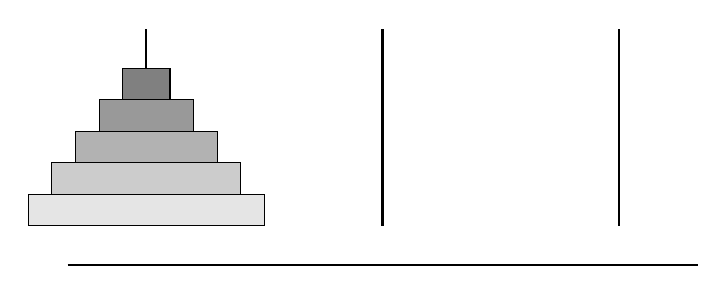
\begin{tikzpicture}
        % Draw the rods
            \draw[thick] (0,0) -- (0,2.5);
            \draw[thick] (3,0) -- (3,2.5);
            \draw[thick] (6,0) -- (6,2.5);
            
        % Draw the base
            \draw[thick] (-1,-0.5) -- (7,-0.5);
            
        % Draw the disks on the first rod
            \draw[fill=gray!20] (-1.5,0) rectangle (1.5,0.4);
            \draw[fill=gray!40] (-1.2,0.4) rectangle (1.2,0.8);
            \draw[fill=gray!60] (-0.9,0.8) rectangle (0.9,1.2);
            \draw[fill=gray!80] (-0.6,1.2) rectangle (0.6,1.6);
            \draw[fill=gray!100] (-0.3,1.6) rectangle (0.3,2);
    \end{tikzpicture}
    \caption{Illustration of the Hanoi Towers problem with disks.}
    \label{fig:hanoi}
\end{figure}

The Hanoi Towers problem consists of three rods and $n$ disks of different sizes. The disks are stacked in decreasing order of size on the first rod. The goal is to move all the disks to the third rod, following the rules:
\begin{itemize}
    \item Only one disk can be moved at a time.
    \item A disk can only be placed on top of a larger disk.
\end{itemize}

Let $h(n)$ be the number of moves required to move $n$ disks from the first to the third rod. The recurrence relation is:
\[
h(n) = 2h(n-1) + 1 = 2(2h(n-2) + 1) + 1 = 2^2 h(n-2) + 2 + 1 =
\]
\[
\dots = 2^n h(0) + 2^{n-1} + 2^{n-2} + \dots + 2^1 + 1
\]
\[
h(n) = 2^n - 1
\]

\subsection{Derangements as recurrence}
\begin{figure}[!h]
    \centering
    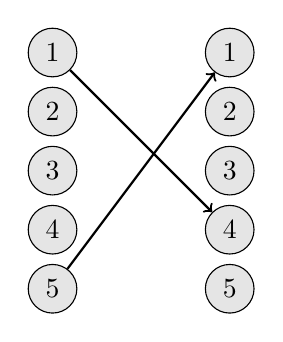
\begin{tikzpicture}[scale=1.5]
        % Nodes on the left
        \foreach \i in {1,2,3,4,5} {
            \node[circle, draw, fill=gray!20, minimum size=0.6cm] (L\i) at (0, 3-\i*0.5) {\i};
        }
        
        % Nodes on the right
        \foreach \i in {1,2,3,4,5} {
            \node[circle, draw, fill=gray!20, minimum size=0.6cm] (R\i) at (1.5, 3-\i*0.5) {\i};
        }
        
        % Arrows
        \draw[->, thick] (L1) -- (R4);
        \draw[->, thick] (L5) -- (R1);
    \end{tikzpicture}
    \label{fig:graph}
    \caption{Graph representation of a derangement.}
\end{figure}
\begin{itemize}
    \item Suppose $4 \rightarrow 1$ \quad $d(n-2)$ ways to derange the remaining elements.
    \item Suppose $4 \nrightarrow 1$ \quad $d(n-1)$ ways to derange the remaining elements.
\end{itemize}
\[
d(n) = (n-1)(d(n-1) + d(n-2))
\]

\subsection*{Example:}
Find a recurrence relation for the number of bit strings of length $n$ that do not contain two consecutive 0s. \\
Consider $n \geq 3$. Build the string from strings of length $n-1$.
\begin{itemize}
    \item If the last digit is 1, there are $d(n-1)$ ways to build the string.
    \item If the last digit is 0, the second-to-last digit must be 1. There are $d(n-2)$ ways to build the string.
\end{itemize}
\[
d(n) = d(n-1) + d(n-2) \quad \text{which is the Fibonacci sequence again!}
\]

\section{Linear Recurrence Relations}
\[
a_n = c_1 a_{n-1} + c_2 a_{n-2} + \dots + c_k a_{n-k} = \left\{a_n\right\}_{n=1}^{\infty}
\]
\[
\text{With } c_i \in \mathbb{R}, \quad c_k \neq 0 \quad \text{and} \quad k \geq 1 = \text{order of the recurrence relation}
\]

\[
1. \quad a_n = r^n, \quad r \in \mathbb{R}, \quad r \neq 0
\]
\[
r^n = c_1 r^{n-1} + c_2 r^{n-2} + \dots + c_k r^{n-k}
\]
\[
r^k - c_1 r^{k-1} - c_2 r^{k-2} - \dots - c_k = 0 \quad \rightarrow \text{Characteristic equation}
\]

\[
2. \quad \text{Superposition principle: the sum of solutions is also a solution} 
\]
\[
\{s_n\}, \{t_n\} \text{ are solutions } \rightarrow \{s_n + t_n\} \text{ is also a solution}
\]

\[
s_n = c_1 s_{n-1} + c_2 s_{n-2} + \dots + c_k s_{n-k}
\]
\[
t_n = c_1 t_{n-1} + c_2 t_{n-2} + \dots + c_k t_{n-k}
\]
\[
s_n + t_n = c_1 (s_{n-1} + t_{n-1}) + c_2 (s_{n-2} + t_{n-2}) + \dots + c_k (s_{n-k} + t_{n-k})
\]

\subsection{The $k = 2$ case}
\[
a_n = c_1 a_{n-1} + c_2 a_{n-2}, \quad c_2 \neq 0
\]
\[
a_0 = \alpha_0, \quad a_1 = \alpha_1, \quad \text{initial conditions}
\]

\[
\text{Then, } \quad r^2 - c_1 r - c_2 = 0
\implies \text{solutions } r_1 \neq r_2
\]

General solution:
\[
a_n = \beta_1 r_1^n + \beta_2 r_2^n
\]

Use the initial conditions to find $\beta_1$ and $\beta_2$.
\[
a_0 = \beta_1 + \beta_2 = \alpha_0 \quad \rightarrow \beta_2 = \alpha_0 - \beta_1
\]
\[
a_1 = \beta_1 r_1 + \beta_2 r_2 = \alpha_1 \quad \rightarrow \alpha_1 = \beta_1 r_1 + (\alpha_0 - \beta_1) r_2
\]

\[
\alpha_1 - \alpha_0 r_2 = \beta_1 (r_1 - r_2) \quad \rightarrow \beta_1 = \frac{\alpha_1 - \alpha_0 r_2}{r_1 - r_2}
\]

\[
\text{Then, } \quad \beta_2 = \alpha_0 - \frac{\alpha_1 - \alpha_0 r_2}{r_1 - r_2} = \frac{\alpha_0 r_1 - \alpha_1}{r_1 - r_2}
\]

\subsection*{Example:}
\[
a_n = a_{n-1} + 2a_{n-2}, \quad a_0 = 2, \quad a_1 = 7
\]
\[
r^2 - r - 2 = 0 \quad \rightarrow r_1 = 2, \quad r_2 = -1
\]
\[
a_n = \beta_1 2^n + \beta_2 (-1)^n
\]

\[
2 = \beta_1 + \beta_2 \quad \rightarrow \beta_2 = 2 - \beta_1
\]
\[
7 = 2 \beta_1 - \beta_2 \quad \rightarrow 7 = 2 \beta_1 - (2 - \beta_1) \quad \rightarrow \beta_1 = 3
\]
\[
\text{Then, } \quad \beta_2 = 2 - 3 = -1
\]

\[
a_n = 3 \cdot 2^n - (-1)^n
\]

\subsection*{Example: Fibonacci sequence}
\[
F_n = F_{n-1} + F_{n-2}, \quad F_0 = 0, \quad F_1 = 1
\]
\[
r^2 - r - 1 = 0 \quad \rightarrow r_1 = \frac{1 + \sqrt{5}}{2}, \quad r_2 = \frac{1 - \sqrt{5}}{2}
\]

\[
0 = \beta_1 + \beta_2 \quad \rightarrow \beta_2 = -\beta_1
\]
\[
1 = \beta_1 \frac{1 + \sqrt{5}}{2} - \beta_1 \frac{1 - \sqrt{5}}{2} \quad \rightarrow \beta_1 = \frac{1}{\sqrt{5}}
\]

\[
F_n = \frac{1}{\sqrt{5}} \left( \left( \frac{1 + \sqrt{5}}{2} \right)^n - \left( \frac{1 - \sqrt{5}}{2} \right)^n \right)
\]

\subsection*{Special case: $r_1 = r_2$}
\[
r^2 - c_1 r - c_2 = 0 \quad \rightarrow \text{With } r_1 = r_2 = r
\]
\[
\text{Then, the general solution is } a_n = \beta_1 r^n + \beta_2 n r^n
\]

\[
a_0 = \beta_1 = \alpha_0 \quad \rightarrow \beta_1 = \alpha_0
\]
\[
a_1 = \beta_1 r + \beta_2 r = \alpha_1 \quad \rightarrow \beta_2 = \frac{\alpha_1 - \alpha_0 r}{r}
\]

\subsection*{Example:}
\[
a_n = 6 a_{n-1} - 9 a_{n-2}, \quad a_0 = 1, \quad a_1 = 6
\]
\[
r^2 - 6r + 9 = 0 \quad \rightarrow r = 3
\]

\[
a_n = \beta_1 3^n + \beta_2 n 3^n
\]
\[
1 = \beta_1 \quad \rightarrow \beta_1 = 1
\]
\[
6 = 3 \beta_1 + 3 \beta_2 \quad \rightarrow 6 = 3 + 3 \beta_2 \quad \rightarrow \beta_2 = 1
\]

\[
a_n = 3^n + n 3^n
\]

\subsection{Theorem: Solution of degree $k$ recurrence relations with constant coefficients}
Let $a_n = c_1 a_{n-1} + c_2 a_{n-2} + \dots + c_k a_{n-k}, \quad c_i \in \mathbb{R}, \quad c_k \neq 0$ be a linear recurrence relation with constant coefficients.
Consider the characteristic equation:
\[
r^k - c_1 r^{k-1} - c_2 r^{k-2} - \dots - c_k = 0
\]
Assume it has different roots $r_1, r_2, \dots, r_t$, with multiplicities $m_1, m_2, \dots, m_t$, with $m_1 + m_2 + \dots + m_t = k$.
Then, the general solution is:

\[
a_n = (\beta_{10} + \beta_{11} n + \beta_{12} n^2 + \dots + \beta_{1m_1} n^{m_1-1}) r_1^n + \dots + (\beta_{t0} + \beta_{t1} n + \beta_{t2} n^2 + \dots + \beta_{tm_t} n^{m_t-1}) r_t^n
\]
\[
a_n = \sum_{i=1}^{t} \sum_{j=1}^{m_i} \beta_{ij} n^{j-1} r_i^n
\]

Given $k$ initial conditions $a_0 = \alpha_0, a_1 = \alpha_1, \dots, a_{k-1} = \alpha_{k-1}$, the coefficients $\beta_{ij}$ can be found by solving the system of linear equations.

\subsection*{Example:}
\[
a_n = -3 a_{n-1} - 3 a_{n-2} - a_{n-3}, \quad a_0 = 1, \quad a_1 = -2, \quad a_2 = -1
\]
\[
r^3 + 3r^2 + 3r + 1 = 0 \quad \rightarrow r = -1, \text{ with multiplicity } 3
\]

\[
a_n = (\beta_1 + \beta_2 n + \beta_3 n^2) (-1)^n
\]
\[
1 = \beta_1 \quad \rightarrow \beta_1 = 1
\]
\[
-2 = (1 + 2 \beta_2 + \beta_3) (-1) \quad \rightarrow 1 = \beta_2 + \beta_3 \quad \rightarrow \beta_2 = 3
\]
\[
-1 = (1 + 2 \beta_2 + 4 \beta_3) \quad \rightarrow -1 = 1 + 2 \beta_2 + 4 \beta_3 \quad \rightarrow \beta_3 = -2
\]

\[
a_n = 1 + 3n - 2n^2 (-1)^n
\]

\subsection{Nonhomogeneous Recurrence Relations}
\[
a_n = c_1 a_{n-1} + c_2 a_{n-2} + \dots + c_k a_{n-k} + F(n)
\]
\[
\text{With } F(n) \text{ a function of } n
\]

\paragraph{Theorem:}
The general solution of the nonhomogeneous case is:
\[
a_n = a_n^{(h)} + a_n^{(p)}
\]

Where $a_n^{(h)}$ is the general solution of the homogeneous case, with $F(n) = 0$, and $a_n^{(p)}$ is a particular solution of the nonhomogeneous case.

\subsection*{Example:}
\[
a_n = 3 a_{n-1} + 2 a_{n-2} + 2^n, \quad a_1 = 3
\]
\[
\text{Homogeneous: } \quad r - 3 = 0 \quad \rightarrow r = 3
\]
\[
\text{General solution: } \quad a_n^{(h)} = \beta 3^n
\]

\[
\text{Particular solution: assume } p_n = cn + d
\]
\[
cn + d = 3(c(n-1) + d) + 2n
\]
\[
cn + d = 3cn - 3c + 3d + 2n
\]
\[
c = 3c + 2 \implies c = -1
\]
\[
d = 3c + 3d \implies d = \frac{-3}{2}
\]

\[
\text{Particular solution: } \quad p_n = -n - \frac{3}{2}
\]
\[
\text{General solution: } \quad a_n = \beta 3^n - n - \frac{3}{2}
\]

\[
a_1 = 3 = \beta 3 - 1 - \frac{3}{2} 
\]
\[
3 \beta = \frac{11}{2} \implies \beta = \frac{11}{6}
\]

\[
a_n = \frac{11}{6} 3^n - n - \frac{3}{2}
\]

\subsection*{Example:}
\[
a_n = 5 a_{n-1} - 6 a_{n-2} + 7^n
\]
\[
r^2 - 5r + 6 = 0 \quad \rightarrow r = 2, 3
\]

\[
a_n^{(h)} = \beta_1 3^n + \beta_2 2^n
\]

\[
p_n = c 7^n = 5(c 7^{n-1}) - 6(c 7^{n-2}) + 7^n
\]
\[
49c = 35c - 6c + 49 \quad \rightarrow 20c = 49 \quad \rightarrow c = \frac{49}{20}
\]

\[
a_n = \beta_1 3^n + \beta_2 2^n + \frac{49}{20} 7^n
\]
\[
a_0 = 1, \quad a_1 = 2
\]

\[
1 = \beta_1 + \beta_2 + \frac{49}{20} \quad \rightarrow \beta_1 + \beta_2 = -\frac{29}{20}
\]
\[
2 = 3 \beta_1 + 2 \beta_2 + \frac{49}{20} \quad \rightarrow 3 \beta_1 + 2 \beta_2 = -\frac{11}{20}
\]
\[
\beta_1 = -\frac{9}{20}, \quad \beta_2 = -\frac{1}{4}
\]

\[
a_n = -\frac{9}{20} 3^n - \frac{1}{4} 2^n + \frac{49}{20} 7^n
\]

\subsection{Theorem: Particular solutions}
Let $a_n = c_1 a_{n-1} + c_2 a_{n-2} + \dots + c_k a_{n-k} + F(n)$ be a linear recurrence relation with constant coefficients and $F(n) = (b_t n^t + b_{t-1} n^{t-1} + \dots + b_1 n + b_0) s^n$.
Then, a particular solution is:
\[
p_n = (d_t n^t + d_{t-1} n^{t-1} + \dots + d_1 n + d_0) s^n
\]

If $s$ is a root of the characteristic equation with multiplicity $m$, then the particular solution is:
\[
p_n = (d_t n^t + d_{t-1} n^{t-1} + \dots + d_1 n + d_0) s^n n^m
\]

\subsection*{Example:}
\[
a_n = 6 a_{n-1} - 9 a_{n-2} + F(n)
\]
\[
F(n) = 3^n, \quad F(n) = n 3^n, \quad F(n) = n^2 2^n, \quad F(n) = (1 + n) 2^n
\]

\[
r^2 - 6r + 9 = 0 \quad \rightarrow r = 3 \text{ with multiplicity } 2
\]

For $F(n) = 3^n$:
\[
p_n = d n^2 3^n
\]

For $F(n) = n 3^n$:
\[
p_n = n^2 (d_1 n + d_0) \cdot 3^n
\]

For $F(n) = n^2 2^n$:
\[
p_n = (d_2 n^2 + d_1 n + d_0) 2^n
\]

For $F(n) = (1 + n) 2^n$:
\[
p_n = n^2 (d_2 n^2 d_1 n + d_0) 3^n
\]


\end{document} 